\documentclass[svgnames,11pt]{beamer}
\input{/home/tof/Documents/Cozy/latex-include/preambule_commun.tex}
\input{/home/tof/Documents/Cozy/latex-include/preambule_beamer.tex}
%\usepackage{pgfpages} \setbeameroption{show notes on second screen=left}
\author[]{Christophe Viroulaud}
\title{Protocole TCP/IP}
\date{\framebox{\textbf{ArchMat 11}}}
%\logo{}
\institute{ Première - NSI }

\begin{document}
\begin{frame}
\titlepage
\end{frame}
\begin{frame}
    \frametitle{}

    Il y a aujourd'hui plusieurs milliards de machines connectés au réseau \emph{Internet}: ordinateurs, smartphones, télévisions, caméras, frigos\dots
\begin{framed}
    \centering Comment faire communiquer plusieurs machines ensembles?
\end{framed}
\end{frame}
\section{Architectures des réseaux}
\begin{frame}
    \frametitle{Architectures des réseaux}

    \begin{center}
    \centering
    \includegraphics[width=9cm]{ressources/local.png}
    \captionof{figure}{\centering Dans un \emph{petit} réseau, les machines sont connectées grâce à un \textbf{switch (connecteur)}.}
    \label{IMG}
    \end{center}

\end{frame}
\begin{frame}
    \frametitle{}
\begin{aretenir}[]
Un \textbf{réseau local} est configuré en \textbf{étoile}, autour d'un \textbf{switch}. C'est une solution peu coûteuse et facile à mettre en place. Mais elle n'est pas adaptée aux réseaux trop importants.
\end{aretenir}
    

\end{frame}
\begin{frame}
    \frametitle{}

    \begin{center}
    \centering
    \includegraphics[width=9cm]{ressources/maille.png}
    \captionof{figure}{\centering Dans un \emph{gros} réseau, les machines sont connectées grâce à un \textbf{routeur}.}
    \label{IMG}
    \end{center}

\end{frame}
\begin{frame}
    \frametitle{}

    \begin{aretenir}[]
    Un \textbf{réseau maillé} utilise plusieurs \textbf{routeurs} disposés en étoile. C'est une solution plus difficile à mettre en place mais plus robuste: en cas de panne d'un routeur, les messages peuvent emprunter un autre chemin.
    \end{aretenir}

\end{frame}
\begin{frame}
    \frametitle{}

    \begin{center}
    \centering
    \includegraphics[width=9cm]{ressources/reseaux.png}
    \captionof{figure}{\centering \textbf{Internet} est appelé le réseau des réseaux.}
    \label{IMG}
    \end{center}

\end{frame}
\section{Histoire de l'Internet}
\begin{frame}
    \frametitle{Histoire de l'Internet}

    \begin{center}
        \centering
        \includegraphics[width=4cm]{ressources/darpa.png}
        \captionof{figure}{\centering \textbf{1967:} La DARPA (défense américaine) développe le concept de réseau informatique. Elle met rapidement en place le réseau \textbf{ARPANET}}
        \label{IMG}
        \end{center}

\end{frame}
\begin{frame}
    \frametitle{}

    \begin{center}
        \centering
        \includegraphics[width=8cm]{ressources/arpanet.png}
        \captionof{figure}{\centering \textbf{Octobre 1972:} Première démonstration publique du réseau ARPANET}
        \label{IMG}
        \end{center}

\end{frame}
\begin{frame}
    \frametitle{}

    \begin{aretenir}[]
        Le réseau ARPANET est composé de:
        \begin{itemize}
            \item 4 nœuds en 1969 (ouest des États-Unis),
            \item 23 nœuds en 1971, 
            \item 111 nœuds en 1974.
        \end{itemize}
        Il relie principalement des universités américaines.
        \end{aretenir}

\end{frame}
\begin{frame}
    \frametitle{}

    \begin{center}
    \centering
    \includegraphics[width=8cm]{ressources/kahncerf.jpg}
    \captionof{figure}{\centering \textbf{1974:} Robert Kahn (droite) et Vinton Cerf (gauche) publient le protocole d'échanges TCP/IP.}
    \label{IMG}
    \end{center}

\end{frame}
\begin{frame}
    \frametitle{}

    \begin{center}
        \centering
        \includegraphics[width=9cm]{ressources/internet.png}
        \captionof{figure}{\centering \textbf{1983:} Le réseau ARPANET est séparé en un réseau militaire et un réseau publique: le terme \textbf{Internet} est adopté.}
        \label{IMG}
        \end{center}

\end{frame}
\section{Le protocole TCP/IP}
\subsection{Présentation}
\begin{frame}
    \frametitle{Le protocole TCP/IP - Présentation}

    \begin{center}
        \begin{tabular}{|c|}
            \hline
            couche application\\
            \hline
            couche transport\\
            \hline
            couche IP\\
            \hline
            couche réseau\\
            \hline
        \end{tabular}
        \captionof{table}{\centering Le protocole est séparé en 4 couches.}
    \end{center}

    \begin{aretenir}[]
    Chaque couche réalise une tâche précise indépendamment des autres.
    \end{aretenir}
\end{frame}
\subsection{Couche réseau}
\begin{frame}
    \frametitle{Couche réseau}

    \begin{aretenir}[]
        La couche réseau transmet l'information \underline{physiquement}:
        \begin{itemize}
            \item par un signal électrique,
            \item par les ondes,
            \item par la lumière.
        \end{itemize}
        \end{aretenir}

\end{frame}
\begin{frame}[fragile]
    \frametitle{}

    \begin{aretenir}[]
    Chaque machine possède une \textbf{adresse MAC (Media Access Control)} unique sur 6 octets; exemple: 47:13:b8:31:07:73
    \end{aretenir}
\begin{center}
\begin{lstlisting}[language=Bash,basicstyle=\ttfamily\small , xleftmargin=1em, xrightmargin=1em]
ip link
\end{lstlisting}
\captionof{code}{Récupérer l'adresse MAC de la carte réseau.}
\label{CODE}
\end{center}
\end{frame}
\begin{frame}
    \frametitle{}

    
    \begin{center}
        \centering
        \includegraphics[width=9cm]{ressources/local.png}
        \captionof{figure}{\centering Le commutateur du réseau local connaît les adresses MAC de chaque machine.}
        \label{IMG}
        \end{center}

\end{frame}
\begin{frame}
    \frametitle{}
\begin{center}
    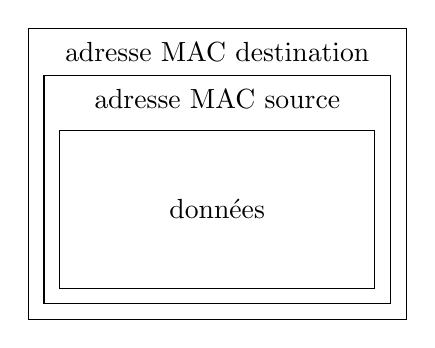
\begin{tikzpicture}
        \draw (-2.2,-1.2) -- (2.2,-1.2) -- (2.2,1.7) -- (-2.2,1.7) -- cycle;  
        \node (mac1) at (0,1.4) {adresse MAC source}; 
        
        \draw (-2.4,-1.4) -- (2.4,-1.4) -- (2.4,2.3) -- (-2.4,2.3) -- cycle;  
        \node (mac2) at (0,2) {adresse MAC destination}; 

        \node[draw,minimum width=4cm,minimum height=2cm,
        rectangle] (donn) at (0,0) {données};
    \end{tikzpicture}
\end{center}

\end{frame}
\end{document}